\documentclass[../main.tex]
		
		\begin{document}
			\section{Review of Propositional Logic}
	\begin{description}
		\item[Task:] Recall enough propositional logic to see how it matches up with set theory.
		\item[Definition:] A \underline{proposition} is any declarative sentence that is either true or false.
	\end{description}
	
	\subsection{Connectives}
	\centerline {
		\begin{tabular}{cccc}
			\multicolumn{3}{c}{\underline{Connectives}} & \multicolumn{1}{c}{\underline{Notation in Maths}} \\
			and & $\land$ \\
			or & $\lor$ & "Inclusive or"\\
			not & $\lnot$ & Sometimes denoted $\sim$\\
			implies & $\to$ & if/then; called implication & $\Rightarrow$\\
			if and only if & $\leftrightarrow$ & Called equivalence & $\Leftrightarrow$\\
		\end{tabular}
	}
	
	\subsubsection{Truth Table of the Connectives}
	Let P, Q be propositions:\\

	\centerline{	
		\begin{tabular}{|c|c|c|}
			\cline{1-3}
			P & Q & P$\land$Q \\ \cline{1-3}
			F & F & F \\ \cline{1-3}
			F & T & F \\ \cline{1-3}
			T & F & F \\ \cline{1-3}
			T & T & T \\ \cline{1-3}
		\end{tabular}
		\quad
		\begin{tabular}{|c|c|c|}
			\cline{1-3}
			P & Q & P$\lor$Q \\ \cline{1-3}
			F & F & F \\ \cline{1-3}
			F & T & T \\ \cline{1-3}
			T & F & T \\ \cline{1-3}
			T & T & T \\ \cline{1-3}
		\end{tabular}
		\quad
		\begin{tabular}{|c|c|}
			\cline{1-2}
			P & $\lnot$P \\ \cline{1-2}
			F & T \\ \cline{1-2}
			T & F \\ \cline{1-2}
		\end{tabular}
		\quad
		\begin{tabular}{|c|c|c|}
			\cline{1-3}
			P & Q & P$\to$Q \\ \cline{1-3}
			F & F & T \\ \cline{1-3}
			F & T & T \\ \cline{1-3}
			T & F & F \\ \cline{1-3}
			T & T & T \\ \cline{1-3}
		\end{tabular}
		\quad
		\begin{tabular}{|c|c|c|}
			\cline{1-3}
			P & Q & P$\leftrightarrow$Q(biconditional) \\ \cline{1-3}
			F & F & T \\ \cline{1-3}
			F & T & F \\ \cline{1-3}
			T & F & F \\ \cline{1-3}
			T & T & T \\ \cline{1-3}
		\end{tabular}
	}
	
	\subsubsection*{Priority of the Connectives}
	\textbf{Highest to Lowest:} $\lnot, \land, \lor, \rightarrow, \leftrightarrow$
	
	\subsection{Important Tautologies}
	\begin{tabular}{rcll}
		$(P \rightarrow Q)$ & $\leftrightarrow$ & $(\lnot P \lor Q)$ \\
		$(P \leftrightarrow Q)$ & $\leftrightarrow$ & $[(P \rightarrow Q) \land (Q \rightarrow P)]$ \\
		$\lnot(P \land Q)$ & $\leftrightarrow$ & $(\lnot P \lor \lnot Q)$ & \multirow{2}{4cm}{\LARGE\} \normalsize De Morgan Laws} \\
		$\lnot(P \lor Q)$ & $\leftrightarrow$ & $(\lnot P \land \lnot Q)$ \\
	\end{tabular}
	~\\~\\~\\
	As a result, $\lnot$ and $\lor$ together can be used to represent all of $\lnot, \land, \lor, \rightarrow, \leftrightarrow$.
	
	\begin{description}
		\item[Less obvious:] One connective called the sheffer stroke P$\mid$Q (which stands for "not both P and Q" or "P nand Q") can be used to represent all of $\lnot$, $\land$, $\lor$, $\rightarrow$, $\leftrightarrow$ since $\lnot$P $\leftrightarrow$ P$\mid$P and P $\lor$ Q $\leftrightarrow$ (P$\mid$P) $\mid$ (Q$\mid$Q).
		\item[Recall] if P$\rightarrow$Q is a given implication, Q$\rightarrow$P is called the \underline{converse} or P$\rightarrow$Q. $\lnot$Q $\rightarrow$ $\lnot$P.
	\end{description}

	\subsection{Logical Equivalences}
	\begin{figure}[!htbp]
		\centering
		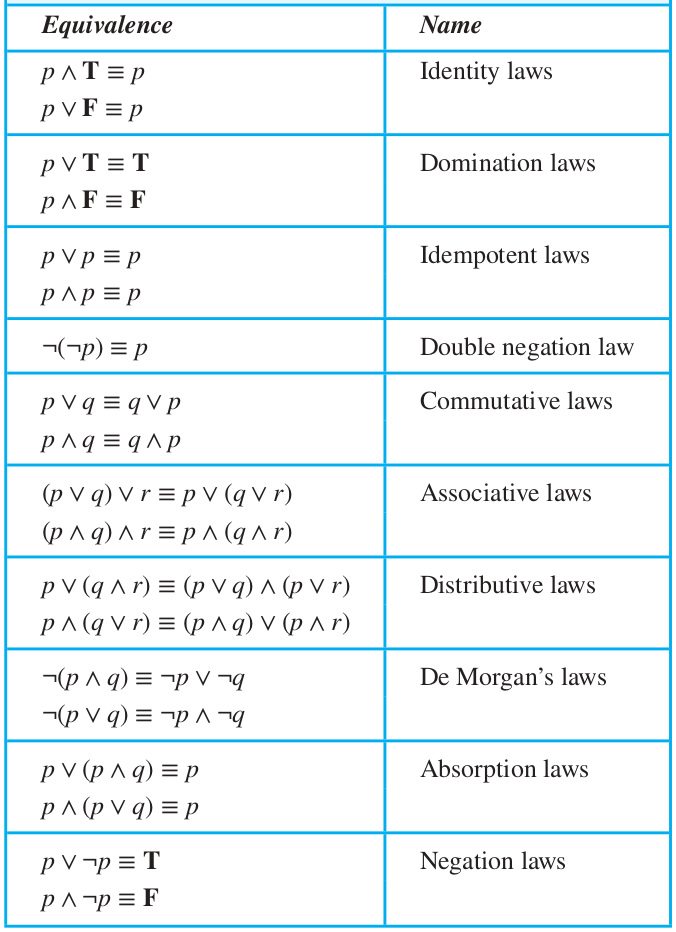
\includegraphics[scale=0.4]{../Figure/pic1.png}
		\caption{Logical Equivalences}
		\end{figure} 
	\begin{figure}[!bthp]
		\begin{minipage}[t]{0.45\linewidth}
		\centering
		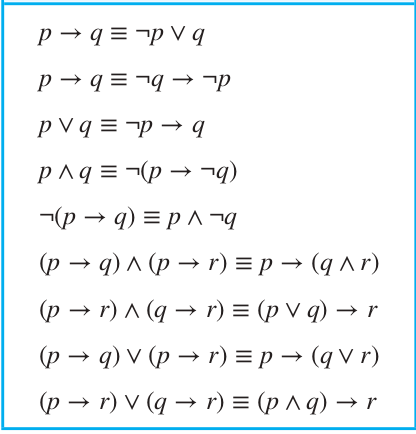
\includegraphics[scale=0.32]{../Figure/pic2.png}
		\caption{Involving Conditional Statements}
		\end{minipage}
		\begin{minipage}[t]{0.45\linewidth}        
		\hspace{2mm}
		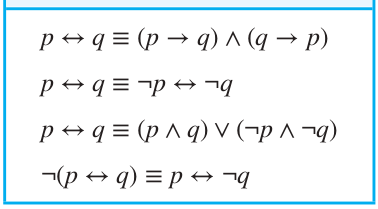
\includegraphics[scale=0.32]{../Figure/pic3.png}
		\caption{Involving Biconditional Statements}
		\end{minipage}
	\end{figure}
	\begin{description}
		\item[De Morgan's Laws:]1.$\lnot (p\vee q) \equiv \lnot p \wedge \lnot q$ ~~~~~2.$\lnot (p\wedge q)\equiv \lnot p\vee \lnot q$ 
	\end{description}

	\subsubsection{Satisfiability}
	\begin{description}
		\item[satisfiable:]if there's an assignment of truth values to its variables that makes it true(tautology/contingency)
		\item[unsatisfiable:]iff. the negation of a compound proposition is tautology
		\item[solution:]an assignment makes a compound proposition true 
	\end{description}

	\subsection{Indirect Arguments/Proofs by Contradiction/Reductio as absurdum}
	Based on the tautology (P$\rightarrow$Q) $\leftrightarrow$ ($\lnot$Q $\rightarrow$ $\lnot$P)
	
	\begin{description}
		\item[Example:] Famous argument that $\sqrt{2}$ is irrational.
		\item[Proof:]
		\item \textbf{Suppose} $\sqrt{2}$ is rational, then it can be expressed is fraction form $\frac{a}{b}$. Let us \textbf{assume} that our fraction is in the lowest term, \textbf{i.e.} their only common divisor is 1.
		\item Then, \[\sqrt{2}=\frac{a}{b}\]
		\item Squaring both sides, we have \[2=\frac{a^2}{b^2}\]
		\item Multiplying both sides by $B^2$ yields \[2b^2=a^2\]
		\item Since $a^2b^2$, we can conclude that $a^2$ is even because whatever the value of $b^2$ has to be multiplied by 2. If $a^2$ is even, then $a$ is also even. Since $a$ is even, no matter what the value of $a$ is, we can always find an integer that if we divide $a$ by 2, it is equal to that integer. If we let that integer be $k$, then $\frac{a}{b}=k$ which means that $a=2k$.
		\item Substituting the value of $2k$ to $a$, we have $2b^2=(2k)^2$ which means that $2b^2=4k^2$. dividing both sides by 2 we have $b^2=2k^2$. That means that the value $b^2$ is even, since whatever the value of $k$ you have to multiply it by 2. Again, is $b^2$ is even, then $b$ is even.
		\item This implies that both $a$ and $b$ are even, which means that both the numerator and the denominator of our fraction are divisible by 2. This contradicts our \textbf{assumption} that $\frac{a}{b}$ has no common divisor except 1. Since we found a contradiction, our assumption is, therefore, false. Hence the theorem is true.
		\item \textbf{qed}
	\end{description}
	

\end{document}